\chapter{实现}
前一章中,我已经详细地描述了本文提出的两个实体链接方法的流程,所以在本章中并没有把太多笔墨放在方法的具体实现上。
在这一章中,我会讲述实验中使用的各类输入数据 (表格,知识库数据) 的来源和处理方法,事实上这些输入数据的规范程度和质量高低决定了实体链接算法能否真正发挥其有效性。
实际上,在实验过程中,我在处理输入数据上花费的时间也远远超过了实现实体链接算法的时间。


\section{表格语料库}
因为基于多知识库的 Web 表格实体链接目前还是一个比较新的任务,几乎没有已知的基准 (Benchmark) 数据集供实验使用。
因此,只能自己来制作基准数据集。
在这里,基准数据集指的是经过人工标注的 Web 表格,用于衡量算法的性能。
对于一个给定的指称,如果算法标注的结果和给定知识库中人工标注的结果相同,那么就认为算法标注的是正确的。
为此,我从 Web 上爬取了超过7万张包含关系型数据的 Web 表格。
然后从中随机挑选了 200 张 Web 表格进行人工标注。
被选中的表格要求包含一定比例的带歧义的指称,为了测试算法的实体消岐能力。
我邀请了4位本科同学一起将表格单元格中的每个字符串指称手动地分别映射到 Zhishi.me 的三个知识库 (中文维基,百度百科和互动百科) 中的实体。
生成了三份表格的人工标注文件,分别对应于三个知识库。
在后续的实验过程中,评估实体链接结果一般是用给定一个知识库对应的人工标注结果来评估,称之为用该知识库来衡量链接结果。
如果要用整个 Zhishi.me 来衡量链接结果,需要将三个知识库的人工标注结果合并。
为了人工标注,我们还开发了一个 Tornado\footnote{\url{http://www.tornadoweb.org}} Web 应用来从网页上标注表格,这种方式直观且高效。
标注结果基于多数投票法,并且是公开的\footnote{\url{https://github.com/yanshengjia/link/tree/master/data}}。


\section{实体知识库}
我采用目前最大的中文百科类知识库 Zhishi.me 作为参考知识库。
换句话说,实验以 Zhishi.me 作为实体的来源。
如图~\ref{zhishime_data} 中所示,Zhishi.me 由三个互有重叠的知识库组成。
这三个知识库是百度百科,互动百科和中文维基百科,它们通过实体间的``sameAs''关系相互链接在一起。
图中的重叠部分代表不同知识库共有的实体。如果来自两个不同知识库的实体间具有``sameAs''关系,这样的实体就是这两个知识库共有的实体。
到目前为止,据统计,在 Zhishi.me 中,百度百科的实体数量最多,为5198298。互动百科其次,为4579805。中文维基百科最少,为559402。
百度百科和中文维基共有实体数量为268592,
中文维基和互动百科共有实体数量为292150,
互动百科和百度百科共有实体数量为3066136,
三个知识库都共有的实体数量为245735,占 Zhishi.me 全部实体数量6956362的3.5\%。
可见不同知识库间共有的实体数量还是相对少的。
另外,Zhishi.me 中共有1.24亿条 RDF 三元组格式的数据,这些数据包含了丰富的关系信息,比如实体与实体之间的关系,实体与属性之间的关系和实体和类别之间的关系。
在我的实验中,需要充分挖掘这些 RDF 三元组数据,来提升实体链接算法的有效性。

\begin{figure}[htbp]
\centering
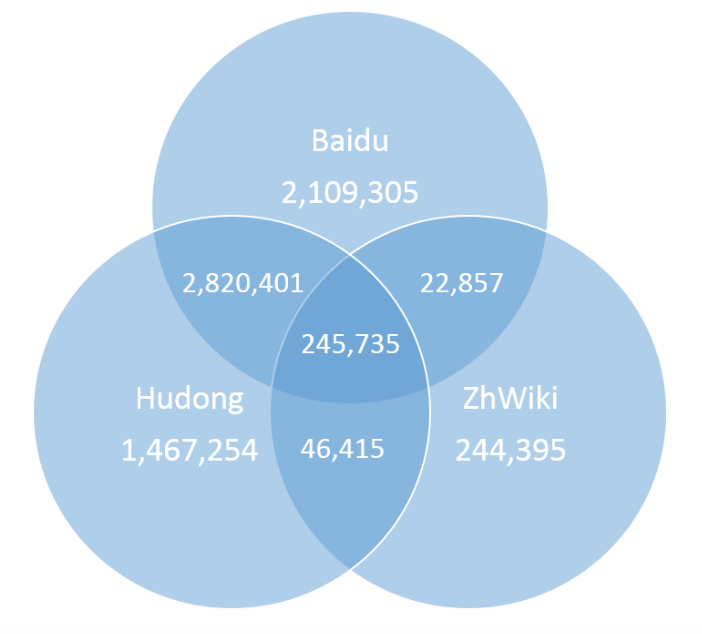
\includegraphics[width=0.4\textwidth]{img/zhishime_data}
\caption{Zhishi.me 数据统计}
\label{zhishime_data}
\end{figure}


\section{数据预处理}
本文中的两个方法接受的输入数据都为结构化的表格数据以及知识库的各类型数据。
在这里,数据预处理分为两个部分,一是对表格数据的预处理,二是对知识库数据的预处理。

1) \textbf{表格数据预处理} \ 
输入表格需要有一个统一的规范的格式:一个 Web 表格表示为一个矩阵,$T$,该表格包含 $r$ 行 $c$列,$T[i,j]$ 代表了 $T$ 在 $i^{th}$ 行和 $j^{th}$ 列的单元格。
而很多 Web 上的表格并不是上述的这种规范化格式,所以需要对表格进行规范化。
表格的规划化主要包括:编码转换,删除多余信息,剔除表头。
有些从 Web 上爬取下来的表格由于编码原因直观上显示得像``乱码''一样,其实这种表格只是使用了某种特殊的编码,比如 unicdoe,只要将这些表格进行编码的转换,转换为 utf8 或者 gbk 编码,表格中的内容应该会显示为中文了。
部分 Web 表格拥有表格说明,一般是表格的编辑人员为了表格的可读性,为表格人工添加了一些解释信息,比如``说明''列或``备注''列,这些多余的表格信息会干扰实体链接算法的性能,在实验中人工将它们剔除。
正如~\ref{contribution} 节中提到,本文中提出的实体链接方法不依赖特定的表头信息,而且我的方法也不对表格的表头进行实体链接,所以要将表格的表头剔除。爬取下来的表格是 HTML 语言表示的,表头一般包含在``<th></th>''标签对中,利用程序定位到该标签对,直接将其剔除。

2) \textbf{知识库数据预处理} \ 
得益于知识库科学与工程实验室的帮助,我直接获取了由实验室爬取的 Zhishi.me 中三个相互链接的知识库的各类数据以及三个知识库间的``sameAs''关系数据。
其中包含了知识库的 labels 数据、abstracts 数据、infobox\_properties 数据、kb1\_kb2\_sameAs 数据等各类数据,它们都是以 RDF 三元组格式存储。
labels 数据就是知识库的实体数据,一般由 unicode 或者 urlcode 编码,需要从每个 RDF 三元组中抽取并转码才能得到实验需要的实体数据。
abstracts 数据代表的是实体在知识库页面中的摘要,在实验中用于生成实体的上下文。
infobox\_properties 数据可以认为是实体的属性,在实验中用于计算 IsRDF 特征和获取实体的上下文。
kb1\_kb2\_sameAs 数据代表着知识库1和知识库2实体之间的``sameAs''关系,也需要抽取并转码才能获取实验需要的``sameAs''关系数据。
这些数据虽然都是以 RDF 三元组格式存储,但是每个数据文件的格式还是有细微差别,同时数据中也存在一定噪声,需要根据文件的格式特点对数据进行抽取和转码以及噪声信息的提出,才能最终得到规范化的高质量的数据。


\section{本章小结}
在本章中,我主要介绍了基于多知识库的实体链接方法的实现。
我并没有过多涉及算法的实现,因为在第三章中已经描述得非常详细了。
我的侧重点主要在于实体链接系统最重要的原材料:数据。
首先,说明了实验使用的基准数据集的来源,然后介绍了实体数据的来源,也就是 Zhishi.me 知识库的各项数据统计,最后对表格数据和知识库数据的预处理方法作了描述。